
% Digital Logic Report Template
% Created: 2020-01-10, John Miller

%==========================================================
%=========== Document Setup  ==============================

% Formatting defined by class file
\documentclass[11pt]{article}

% ---- Document formatting ----
\usepackage[margin=1in]{geometry}	% Narrower margins
\usepackage{booktabs}				% Nice formatting of tables
\usepackage{graphicx}				% Ability to include graphics

%\setlength\parindent{0pt}	% Do not indent first line of paragraphs 
\usepackage[parfill]{parskip}		% Line space b/w paragraphs
%	parfill option prevents last line of pgrph from being fully justified

% Parskip package adds too much space around titles, fix with this
\RequirePackage{titlesec}
\titlespacing\section{0pt}{8pt plus 4pt minus 2pt}{3pt plus 2pt minus 2pt}
\titlespacing\subsection{0pt}{4pt plus 4pt minus 2pt}{-2pt plus 2pt minus 2pt}
\titlespacing\subsubsection{0pt}{2pt plus 4pt minus 2pt}{-6pt plus 2pt minus 2pt}

% ---- Hyperlinks ----
\usepackage[colorlinks=true,urlcolor=blue]{hyperref}	% For URL's. Automatically links internal references.

% ---- Code listings ----
\usepackage{listings} 					% Nice code layout and inclusion
\usepackage[usenames,dvipsnames]{xcolor}	% Colors (needs to be defined before using colors)

% Define custom colors for listings
\definecolor{listinggray}{gray}{0.98}		% Listings background color
\definecolor{rulegray}{gray}{0.7}			% Listings rule/frame color

% Style for Verilog
\lstdefinestyle{Verilog}{
	language=Verilog,					% Verilog
	backgroundcolor=\color{listinggray},	% light gray background
	rulecolor=\color{blue}, 			% blue frame lines
	frame=tb,							% lines above & below
	linewidth=\columnwidth, 			% set line width
	basicstyle=\small\ttfamily,	% basic font style that is used for the code	
	breaklines=true, 					% allow breaking across columns/pages
	tabsize=3,							% set tab size
	commentstyle=\color{gray},	% comments in italic 
	stringstyle=\upshape,				% strings are printed in normal font
	showspaces=false,					% don't underscore spaces
}

% How to use: \Verilog[listing_options]{file}
\newcommand{\Verilog}[2][]{%
	\lstinputlisting[style=Verilog,#1]{#2}
}




%======================================================
%=========== Body  ====================================
\begin{document}
	
	\title{ELC 2137 Lab 03: Adders}
	\author{Yiting Wang}
	
	\maketitle
	
	
	\section*{Summary}
	
		Logic circuits began as discrete components, which were then packaged into “integrated circuits” (ICs or “chips”) that might contain several individual gates or more complicated circuits. The goals of this Lab are to be able to design logical circuits that implement a desired function, and introduces a family of logic “chips” (integrated circuits or ICs) that can be used to design simple logic circuits.\\
	
	
	
	\section*{Q\&A}
	
	\begin{enumerate}
		\item Which gates could we use for combining the carry bits? Which one should we use and why?\\
			We should use XOR gate. When there are two 1’s as inputs, we need to cut off 1 bit; and when there are 0's and 1’s as inputs, we need to keep that. An XOR gate will give you a 0 with two 1’s as inputs, and a 1 with one 1's as input.\\
	\end{enumerate}
	
	
	
	\section*{Results}	
	
	Figure 1 is the cricuit domonstration page. It has the HA and FA schematics and wiring diagrams, and three instructor signatures.\\
	\begin{figure}[ht]\centering
		\includegraphics[width=0.7\textwidth]{Lab3Page}
		\caption{The Circuit Demonstration Page}
		\label{fig:Lab3Page}
	\end{figure}
	
	Figure 2 is the picture of my Half Adder circuit, I built it based on the Half Adder wiring diagrams I draw on the cricuit domonstration page.\\
	\begin{figure}[ht]\centering
		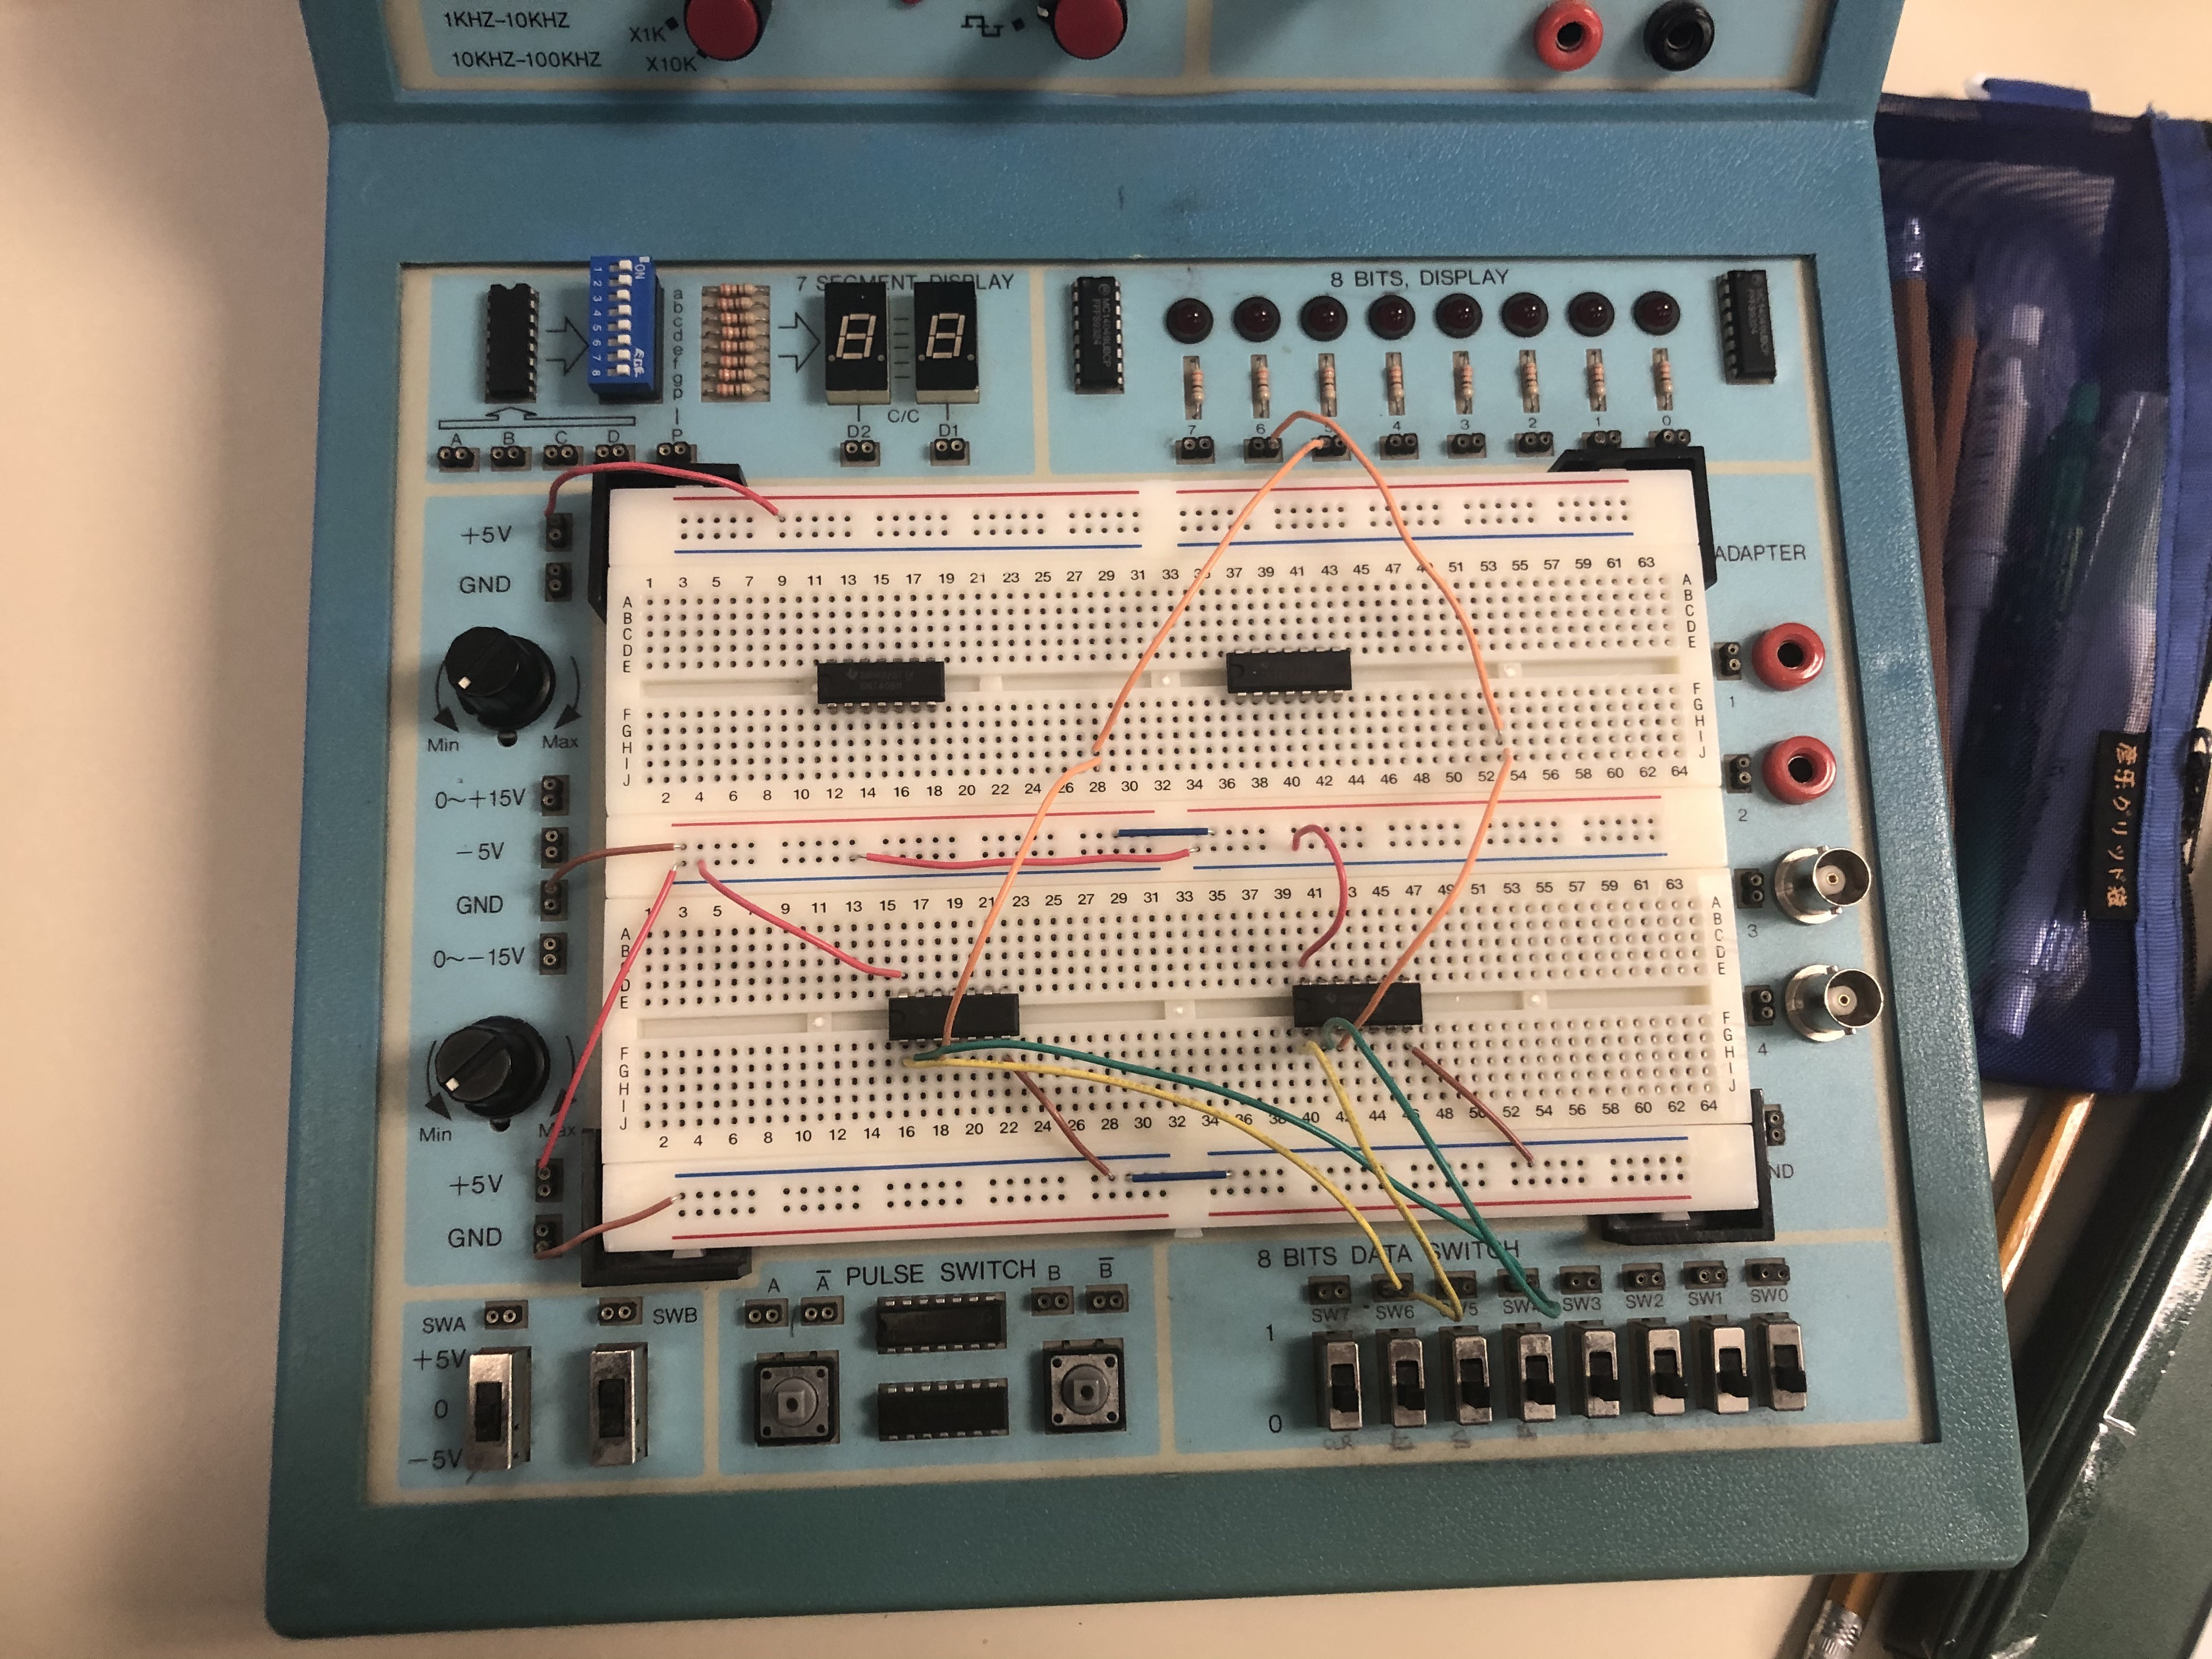
\includegraphics[width=1.0\textwidth,trim=20cm 15cm 20cm 15cm,clip]{HalfAdder}
		\caption{The Half Adder Circuit}
		\label{fig:HalfAdder}
	\end{figure}

	 Figure 3 is the picture of my Full Adder circuit, I built it based on the Full Adder wiring diagrams I draw on the cricuit domonstration page.\\
	\begin{figure}[ht]\centering
		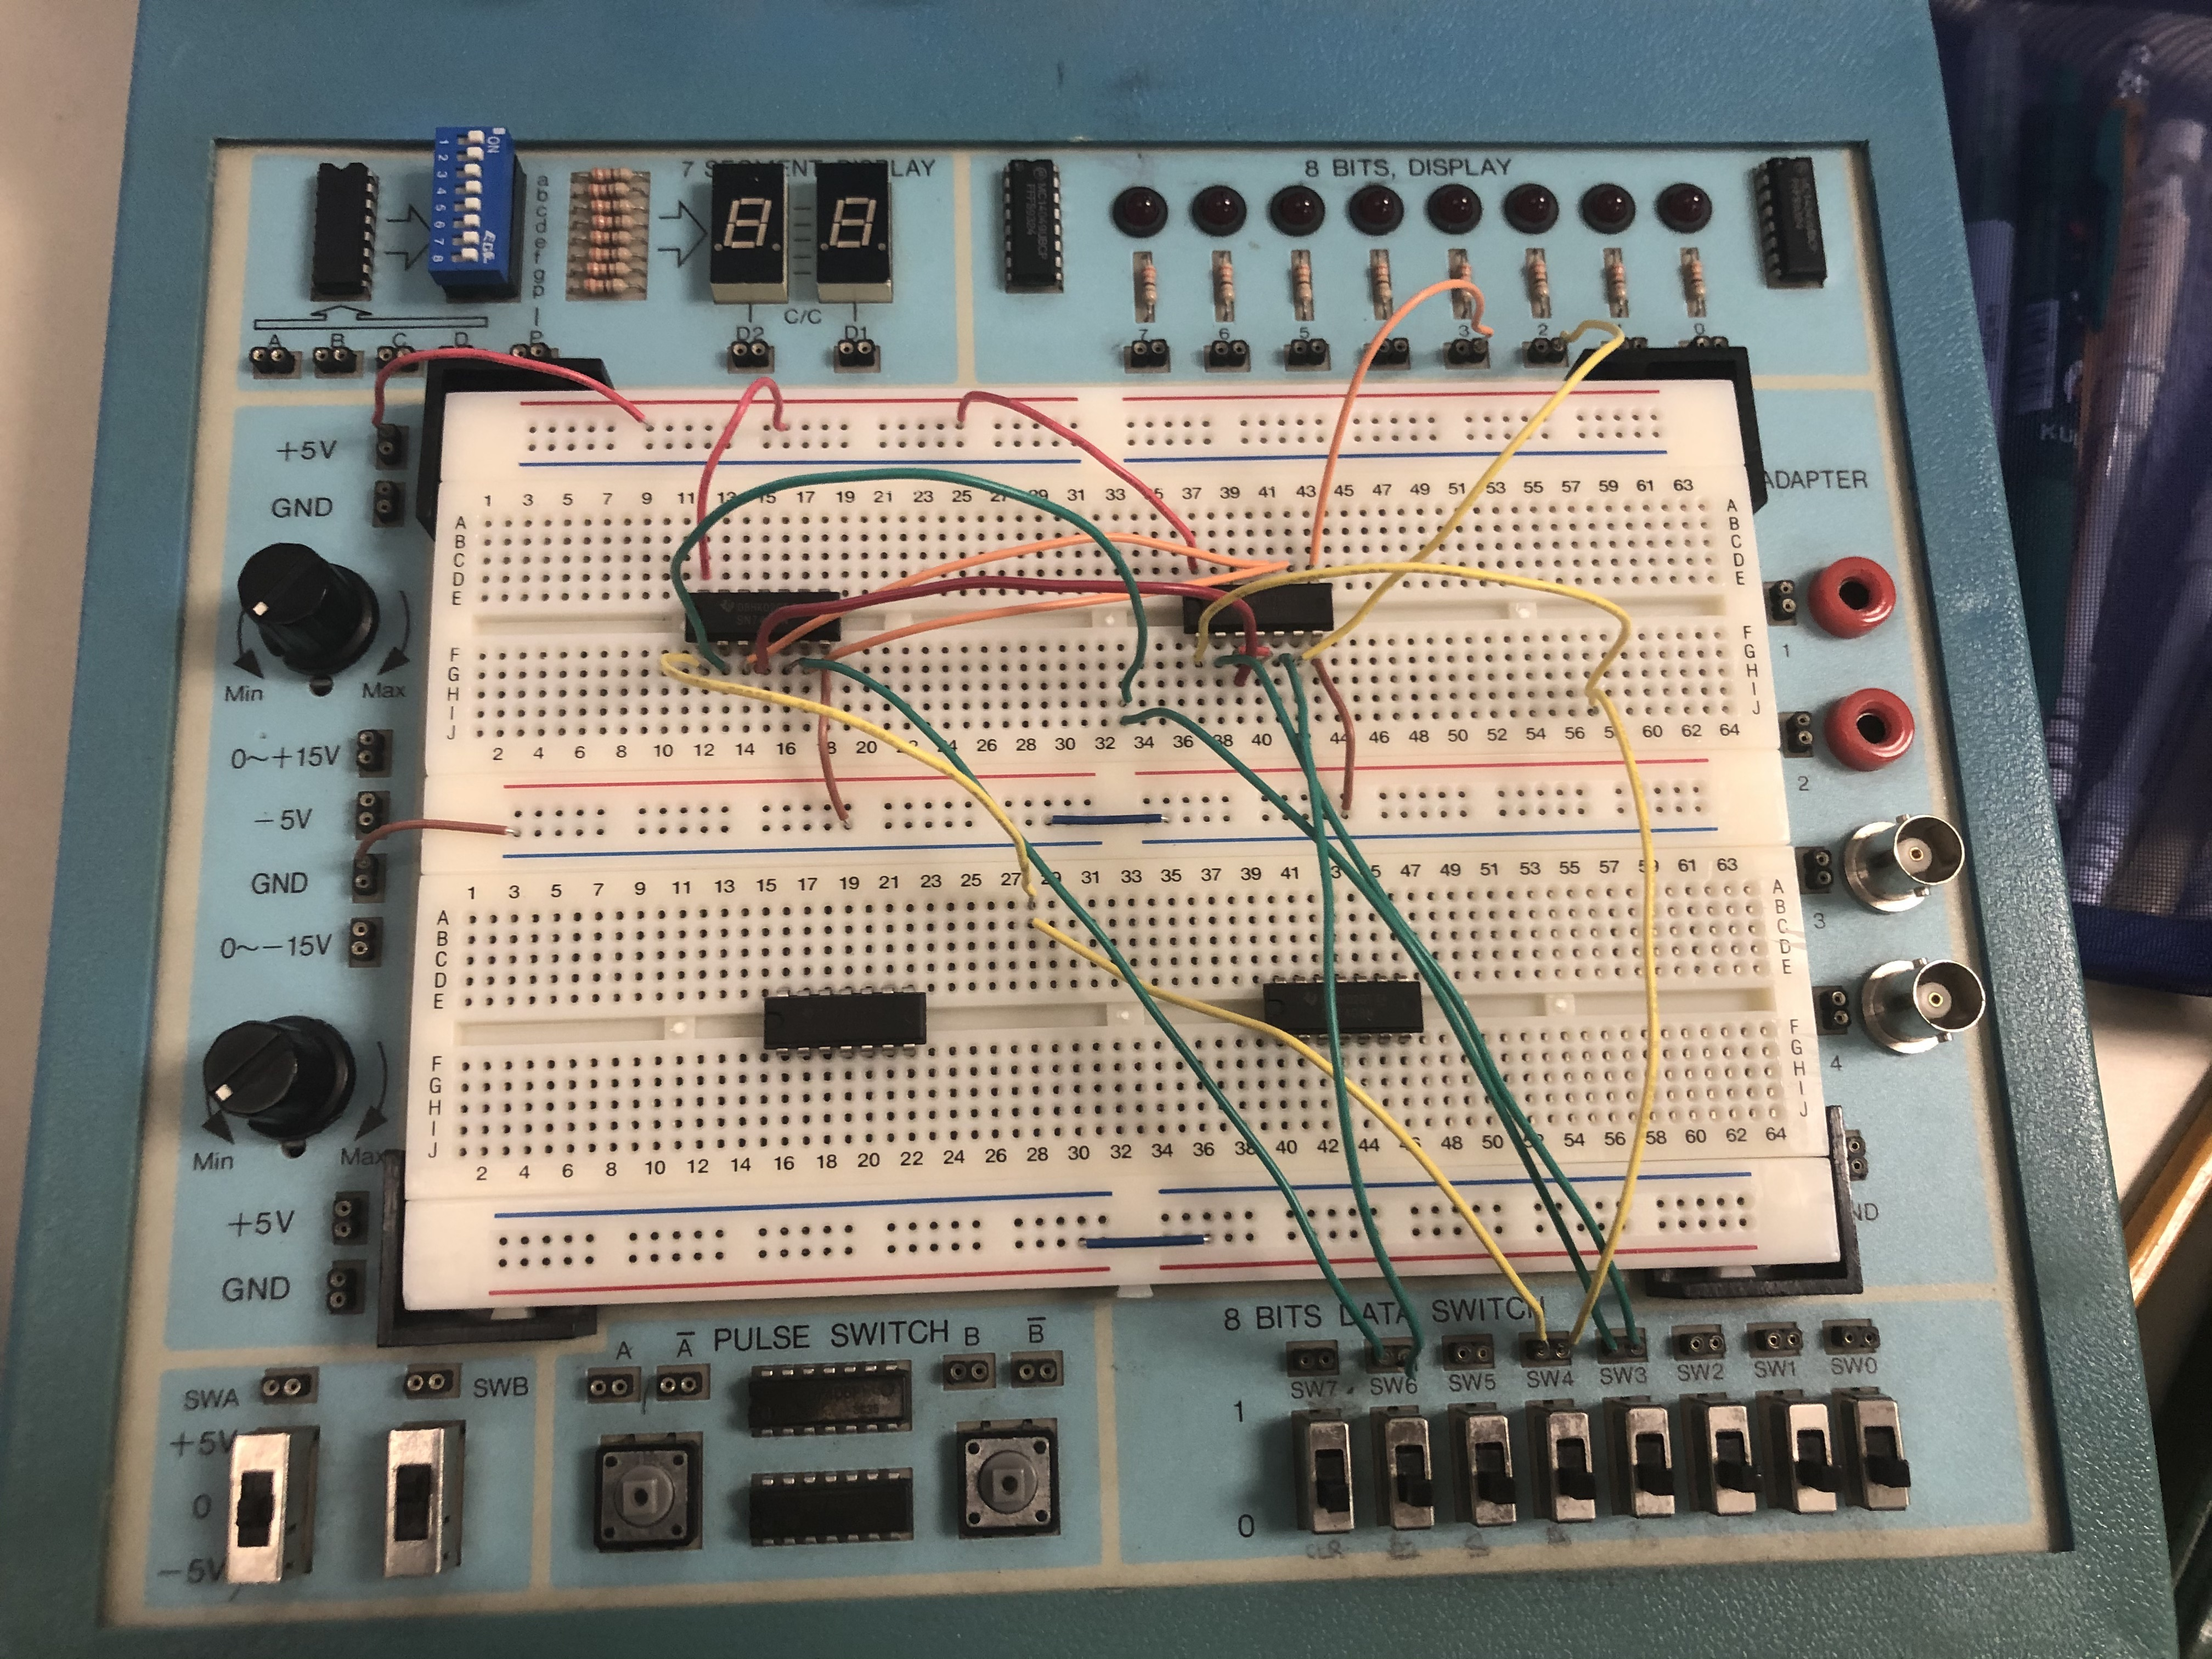
\includegraphics[width=1.0\textwidth]{FullAdder}
		\caption{The Full Adder Circuit}
		\label{fig:FullAdder}
	\end{figure}

	 Figure 4 is the picture of my 2-bit Adder circuit, I built it based on the 2-bit Adder instruction. I built 2 working Full Adders, I connected the carry output of one adder to the carry input of the other adder (instead of a switch).\\
	\begin{figure}[ht]\centering
		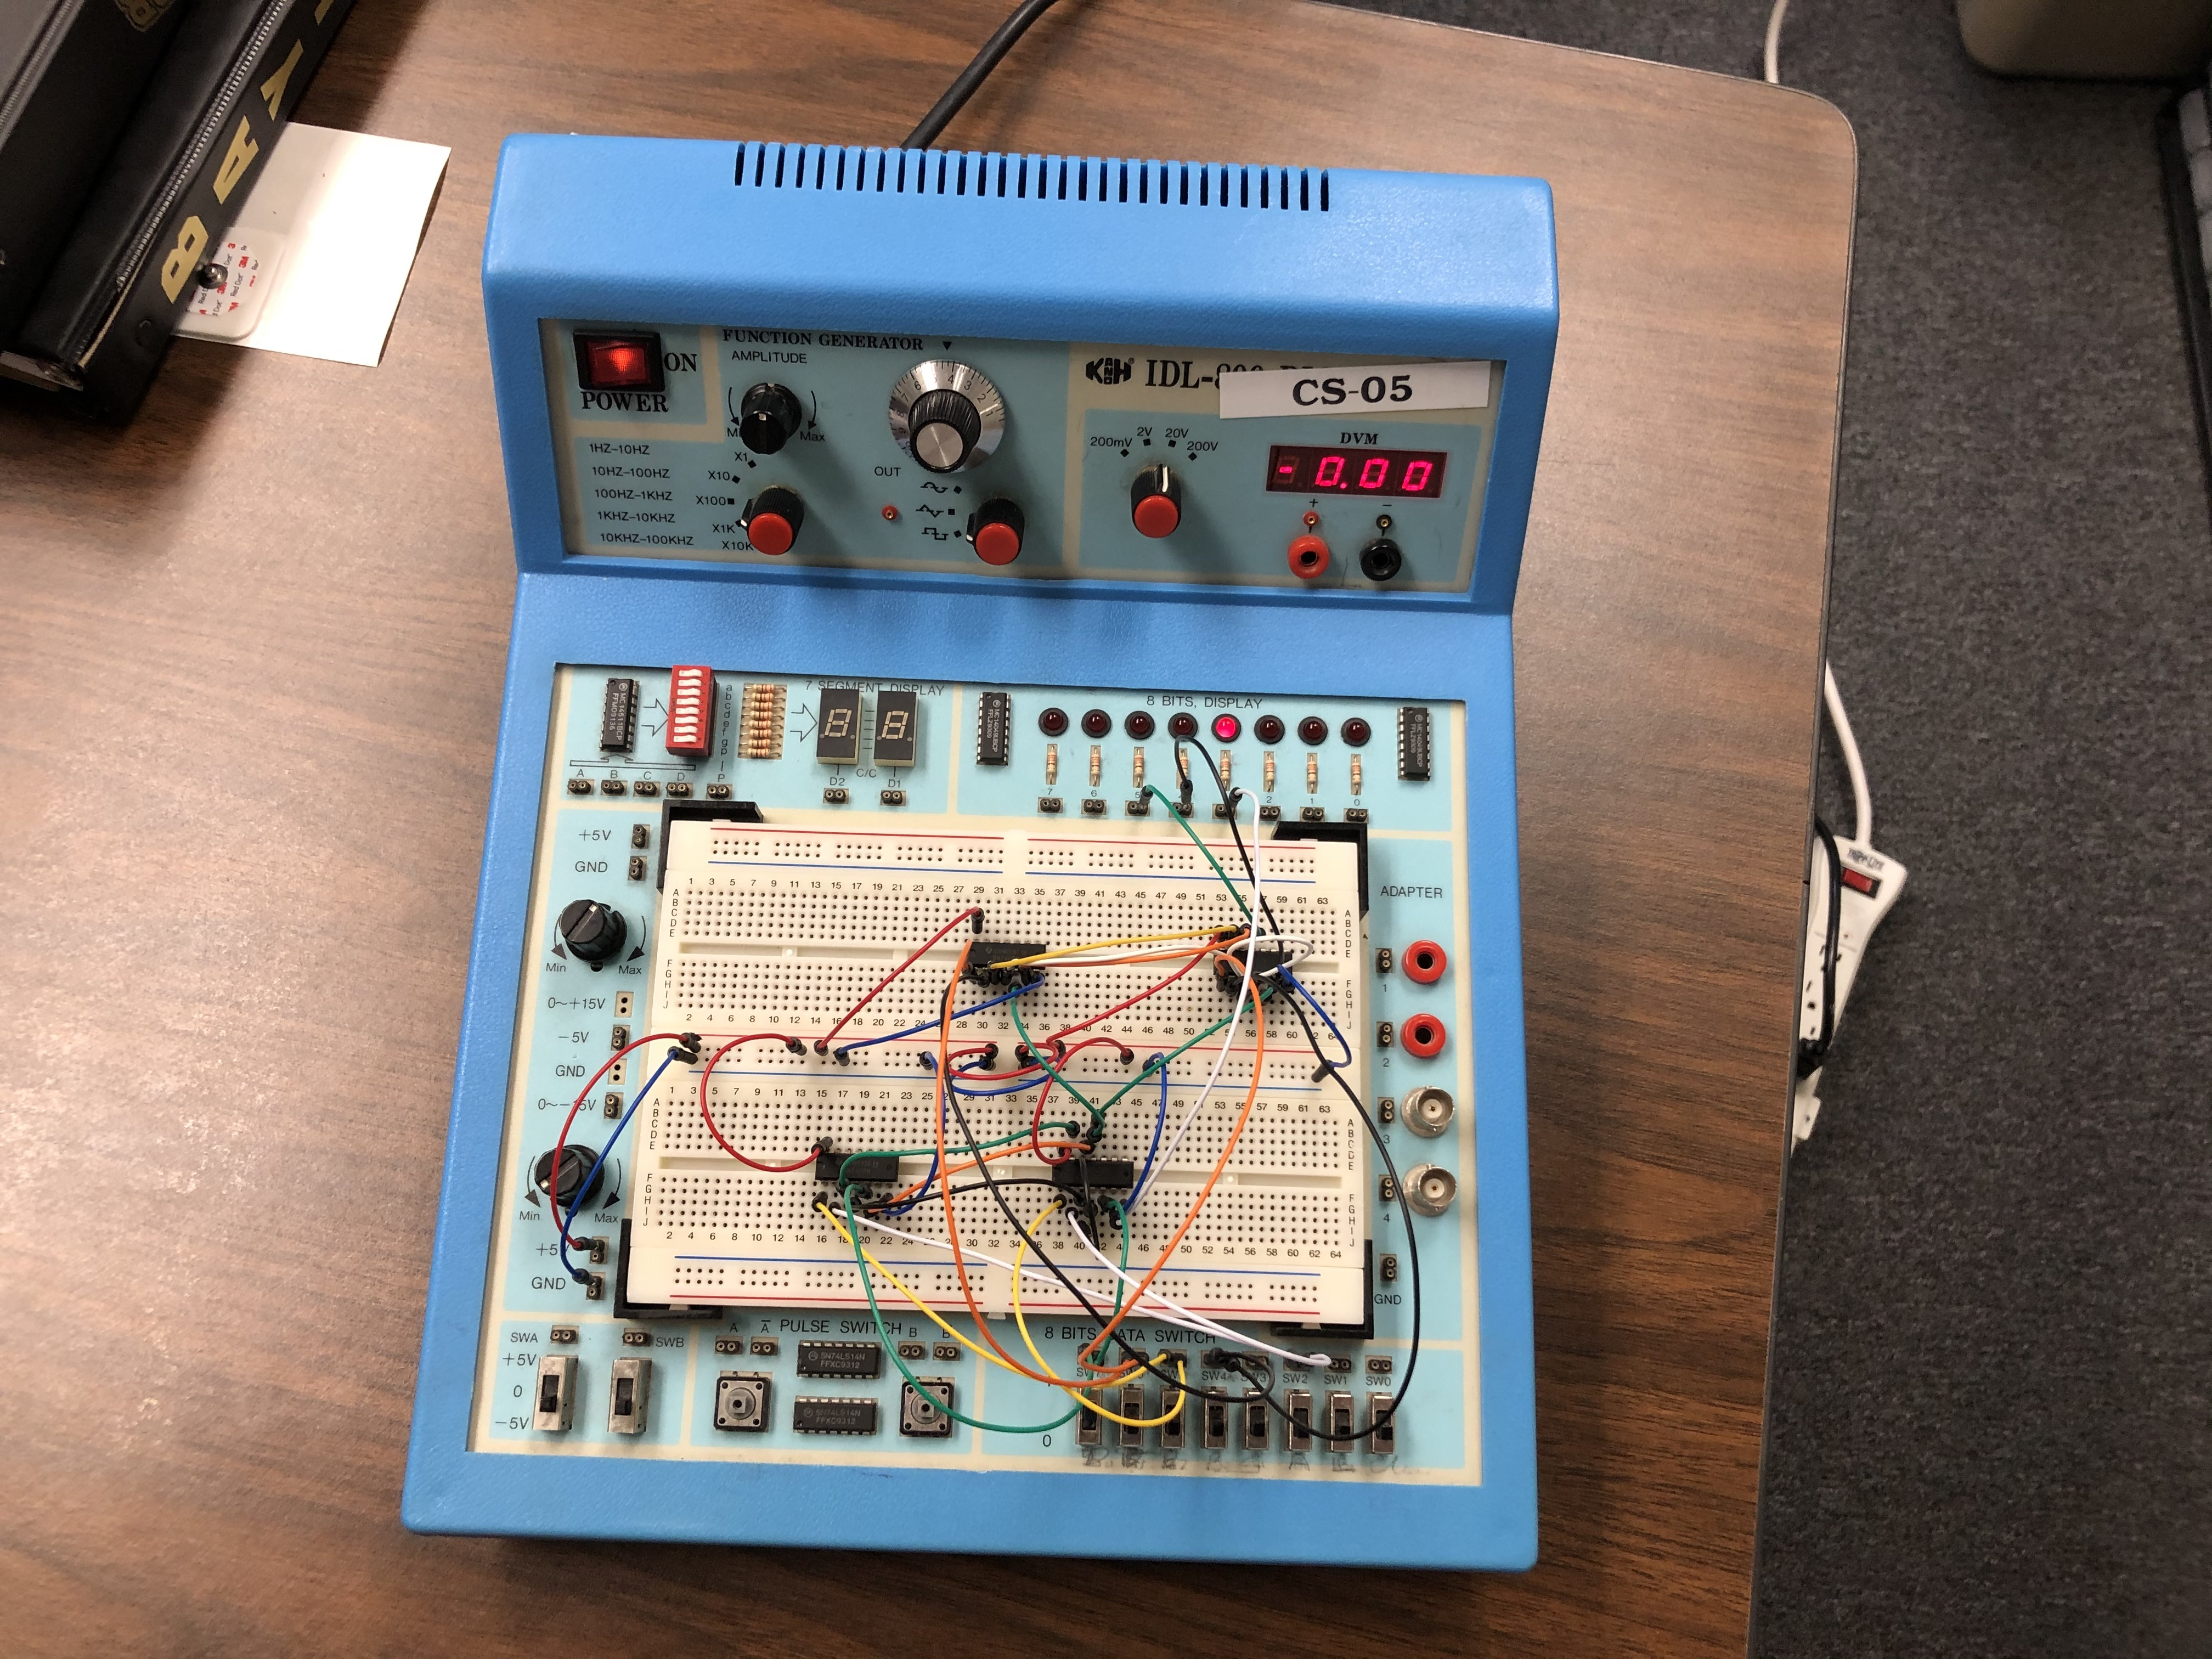
\includegraphics[width=1.0\textwidth,trim=30cm 10cm 40cm 40cm,clip]{2-bitAdder}
		\caption{The 2-bit Adder Circuit}
		\label{fig:2-bitAdder}
	\end{figure}
	
	Table 1 is the Full Adder's expanded truth table. I did this table based on these: c1 = A and B; s1 = A xor B; c2 = s1 and Cin; S = s2 = s1 xor Cin; Cout = c1 xor c2. This table also proofs that the carry outputs of the first and sec-ond stage HAs cannot both be high at the sametime.\\
	\begin{table}[ht]\centering
		\caption{FA expanded truth table}
		\label{tbl:FA expanded truth table}
		\begin{tabular}{ccc|cccc|cc}
			\toprule
			Cin & A & B & c1 & s1 & c2 & s2 & Cout & S \\
			\midrule
			0 & 0 & 0 & 0 & 0 & 0 & 0 & 0 & 0 \\
			0 & 0 & 1 & 0 & 1 & 0 & 1 & 0 & 1 \\
			0 & 1 & 0 & 0 & 1 & 0 & 1 & 0 & 1 \\
			0 & 1 & 1 & 1 & 0 & 0 & 0 & 1 & 0 \\
			\midrule
			1 & 0 & 0 & 0 & 0 & 0 & 1 & 0 & 1 \\
			1 & 0 & 1 & 0 & 1 & 1 & 0 & 1 & 0 \\
			1 & 1 & 0 & 0 & 1 & 1 & 0 & 1 & 0 \\
			1 & 1 & 1 & 1 & 0 & 0 & 1 & 1 & 1 \\
			\bottomrule
		\end{tabular}
	\end{table}
	
	
	
	\section*{Code}
	
	There is no code require in this lab.\\	
	
	
		
\end{document}